\chapter{Testing Procedures}
\label{ch:testing-procedures}

In previous chapters we introduced an approach for estimating certain key metrics about a population based on a sample, for example using point estimators or confidence intervals.
We can also use this information to test certain hypotheses about a population. A hypothesis is an assumption that has yet to be proven.
The purpose of a testing procedure is to test a hypothesis regarding the value of 1 or more population parameters.

\begin{definition}[Statistical Hypothesis]
  A statistical hypothesis\index{hypothesis!statistical} is a statement about the numerical value of a population parameter.
\end{definition}

Examples of hypotheses:

\begin{itemize}
  \item On average, a superhero rescues at least 3.3 people a day.
  \item The average height of a superhero is at least 120 cm.
  \item \dots
\end{itemize}

In this chapter we will formulate the general theory of testing using hypotheses about the population mean $\mu$, the $Z$-test.
Apart from the $Z$-test, there are many other statistical hypothesis tests that can be used in specific cases.
The most appropriate statistical test depends, among other things, on the population size in question (average, standard deviation, etc.),
and assumptions regarding the underlying stochastic distribution of the population (normally distributed or not, etc.).

\section{Learning Goals}
\label{sec:testing-procedures-learning-goals}

By the end of this chapter you must be able to:

\begin{itemize}
  \item Explain the following concepts:
  \begin{itemize}
    \item hypothesis test, statistical hypothesis, null hypothesis, alternative hypothesis;
    \item test statistics, region of acceptance, region of rejection / critical region, probability value;
    \item $Z$-test, $t$-test, left tail, right tail, two tail;
    \item Type I and Type II errors;
  \end{itemize}
  \item Describe the general procedure for a statistical test;
  \item Based on the description of a situation in which you are asked to verify a statement about the population mean:
  \begin{itemize}
    \item to determine whether a $z$- or $t$-test could be used;
    \item to deduce from the research question whether the left, right of two tail variant should be used;
  \end{itemize}
  \item To correctly apply the $z$- or $t$-test for a given situation, i.e.:
  \begin{itemize}
    \item Formulate the null and alternative hypotheses (mathematical notation);
    \item Calculate the test statistic
    \item Calculate the critical value(s) and determine whether the test statistic is inside the region of acceptance or rejection;
    \item Calculate the probability value;
    \item Formulate a correct conclusion (reject null hypothesis or not);
    \item Formulate an answer to the research question.
  \end{itemize}
\end{itemize}

\section{Elements of a hypothesis test}
\label{sec:elements-hypothesis-test}

In general, a testing procedure consists of 4 elements:
\begin{enumerate}
  \item \textbf{Null Hypothesis}\index{null hypothesis}\index{hypothesis!null} $H_{0}$: We will try to disprove this hypothesis using proof by contradiction. We will accept this hypothesis, unless observations from the sample convincingly point to the contrary.
  \item \textbf{Alternative hypothesis}\index{hypothesis!alternative} $H_{1}$: In general, this is the hypothesis the researcher wants to prove. However, this hypothesis will only be accepted if the observations from the sample convincingly indicate its correctness.
  \item \textbf{Test Statistic}: The variable that is derived from the sample
  \item Region of acceptance and region of rejection / critical region:
  \begin{itemize}
    \item \textbf{Region of Acceptance\index{region of acceptance}}: The region of values supporting the null hypothesis $H_{0}$
    \item \textbf{Region of Rejection\index{region of rejection}}: The region containing the values that reject the null hypothesis. Also referred to as critical region\index{region!critical}.
  \end{itemize}
\end{enumerate}

An alternative for the last step is calculating the \emph{probability value} (see further).

The decision to reject or accept the null hypothesis $H_{0}$ is based on information from a sample, drawn from a population on which the hypothesis is based.
The sample values are used to calculate a single value of a test statistic that will determine the decision. 
To this end, all possible values for the test statistic are divided into two regions, the region of acceptance and the region of rejection.
If the value of the test statistic is inside the region of rejection, the null hypothesis is rejected and the alternative hypothesis accepted.
If the value of the test statistis is inside the region of acceptance, the null hypothesis is accepted.

\section{Testing Procedure for the \texorpdfstring{$z$}{z}-test}
\label{sec:testing-procedure-z-test}

For the first test procedure we will discuss in this course, we will verify a statement about the population mean $\mu$.
This test procedure is commonly known as the $Z$-test\index{$Z$-test}\index{test!$Z$}.

\begin{enumerate}
  \item The suspicions about the population are described using two hypotheses $H_{0}$ and $H_{1}$. For the (right-tail) $Z$-test the null hypothesis states that the population mean $\mu$ has a certain value, and the alternative hypothesis states that $\mu$\ is \emph{greater} than this value.
  \item The significance level\index{significance level}\index{level!significance} $\alpha$ and sample size $n$ are determined. In principle, you can choose a value for $\alpha$ (e.g. 0.05)\footnote{Note that the significance level is related to the confidence interval $1-\alpha$, cfr. Section~\ref{ssec:confidence-interval-pop-mean-large-sample}}. The closer the significance level is to 0, the less doubt there is about the result of the test, but on the other hand it becomes more difficult to reject the null hypothesis.
  \item The value of the test statistic for the sample is calculated. The result determines whether we can reject the null hypothesis $H_{0}$ or not. Thanks to the central limit theorem we know that the probability distribution of the sample mean is normally distributed, $M \sim Nor( \mu, \frac{\sigma}{\sqrt{n}})$.
  \item We determine the critical region, or more specifically the boundary between the region of acceptance and the region of rejection. We look for a critical value $g$ so that:
  
  \begin{align}
  P(M > g) = \alpha & \Leftrightarrow P\left(Z> z=\frac{g-\mu}{\sigma/\sqrt{n}}\right) = \alpha & \mathrm{(standardization)}\\
  & \Leftrightarrow P\left(Z < z = \frac{g-\mu}{\sigma/\sqrt{n}}\right) = 1-\alpha & \mathrm{(100\%-rule)}
  \end{align}
  
  The $z$-value depends on the chosen significance level, and can be found using a $z$-table or calculated using the R function \texttt{qnorm(1-alpha)}. From this we can derive $g$:
  
  \begin{equation}
  z = \frac{g-\mu}{\sigma/\sqrt{n}} \Leftrightarrow g = \mu + z \frac{\sigma}{\sqrt{n}}
  \label{eq:critical-calue-z-test}
  \end{equation}

  All values \emph{left} of $g$ form the region of acceptance. Value on the right, which are far away from the assumed population mean $H_0$, form the region of rejection, cfr. Section~\ref{sec:critical-region}.
\end{enumerate}

\begin{example}
  \label{ex:hypothesis-test-daily-rescues}
  In general we assume that superheroes rescue 3.3 people per day on average. However, researchers are getting the feeling that this is not the case: they have the impression that a superhero rescues \emph{more} than $3.3$ people per day.

  The researchers want to to investigate this and take a sample of $n = 30$ superheroes. For this sample, the sample mean is $\overline{x} = 3,483$. The standard deviation of the population is assumed to be known and is equal to $\sigma = 0.55$.
  
  Using these results, can the researchers conclude that superheroes rescue on average more than 3.3 people per day?

  \begin{enumerate}
    \item We assume that the number of people a superhero rescues on average is normally distributed and formulate two hypotheses regarding the parameter $\mu$.
    \begin{itemize}
      \item $H_{0}$ = the null hypothesis (that we want to reject). In this case: \[ H_{0} : \mu = 3.3 \]
      \item $H_{1}$ = alternative hypothesis (suspect that we want to prove). In this case: \[H_{1}= \mu > 3.3 \]
    \end{itemize}
  
    We initially assume that the null hypothesis $H_{0}$ is true. If the average number of people rescued per day of the sample ($\overline{x}$) differs a lot from the assumed value, we reject the null hypothesis $H_{0}$ and accept the alternative hypothesis $H_{1}$.

    But how do we define ``differs a lot''? Would it be easy to draw a sample with a mean of $3.483$ based on a population with a mean of $3.3$? The central limit theorem (cfr. Section~\ref{ch:central-limit-theorem}) allows for calculating the probability of this.
    
    \item Determine significance level $\alpha$ and sample size $n$. We want to have a significance level of 5\%, so $\alpha = 0.05$. The sample size is provided for this case, and is equal to $n = 30$.
    
    \item Calculate the value of the test statistic in the sample. For this example, we take the sample mean: $\overline{x} = 3.483$
    
    We assume that the null hypothesis $H_{0}$ is true and that we have a good estimate for $\sigma$ ($\sigma = 0,55$). Then, according to the central limit theorem, we can say about the sample mean $M$ that:

    \[M \sim  Nor(\mu = 3.3; \sigma = \frac{0.55}{\sqrt{30}})\]

    The value $\overline{x} = 3,483$ is located on the far right (see Figure~\ref{fig:hypothesis-test-daily-rescues}). $\overline{x} $ is so far to the right that the probability to get this or a greater value, is very small (if $H_{0}$ is true). As a result, it is very difficult to explain such a value based on mere coincidence. Intuitively we feel that the further the observed value of $\overline{x}$ is located in the right direction, the more inclined we are to reject the null hypothesis. But what is too far and what is not?
    
    \item Calculate the critical value. The $z$=value for a significance level of $0,05$ equals 1.654\footnote{This can be calculated in R using \texttt{qnorm(1 - 0.05)}}.
    
    \[ g = \mu + z \times \frac{\sigma}{\sqrt{n}} = 3.3 + 1.645 \times \frac{0.55}{\sqrt{30}} \approx 3.45 \]
    
    The sample mean $\overline{x} = 3.483 $ is even further away from $\mu = 3.3$ than the limit value $g = 3.45$. It is therefore very unlikely that such a sample can be drawn from a population with this average. Such an event will only occur in 34 samples out of 1000. In other words, the sample value is in the rejection area. Because of this, we can reject $H_0$ and conclude that superheroes indeed rescue \emph{more} than 3.3 people a day.

  \end{enumerate}

\end{example}

\begin{exercise}
  Can we assume in Example~\ref{ex:hypothesis-test-daily-rescues} that the mean has a normal distribution? Why (not)?
\end{exercise}

\begin{figure}
  \centering
  \begin{tikzpicture}
    \begin{axis}[
        domain=3:3.6, samples=100,
        axis lines*=left, xlabel=$x$,
        every axis y label/.style={at=(current axis.above origin),anchor=south},
        every axis x label/.style={at=(current axis.right of origin),anchor=west},
        height=5cm, width=12cm,
        xtick={3.3,3.483}, ytick=\empty,
        xticklabels={$\mu$,$\overline{x}$},
        enlargelimits=false, clip=false, axis on top,
        grid = minor
      ]
      \addplot [fill=cyan!20, draw=none, domain=3:3.465] {gauss(3.3,0.1004)} \closedcycle;
      \addplot [fill=none, draw=black, domain=3:3.6] {gauss(3.3,0.1004)} \closedcycle;
      \draw [-](axis cs:3.465,1.6) -- (axis cs:3.465,0);
      \node at (axis cs:3.465,1.8) {3.465};
      \node at (axis cs:3.483,-0.7) {3.483};
      \node at (axis cs:3.3,-0.7) {3.3};
    \end{axis}
  \end{tikzpicture}
  \caption{Distribution of the number of people rescued by a superhero on average per day (Example~\ref{ex:hypothesis-test-daily-rescues}). The probability distribution of the sample mean is normally distributed with $\mu = 3.3$ and $\sigma = 0.55$. The sample mean is $\overline{x} = 3.483$. The critical value for acceptance/recjection of $H_{0}$ is 3.465.}
  \label{fig:hypothesis-test-daily-rescues}
\end{figure}

\section{Critical Region}
\label{sec:critical-region}

The formula for calculating the critical value (cfr. Equation~\ref{eq:critical-calue-z-test}) is based on the central limit theorem, and in particular on confidence intervals.

The critical value defines a confidence interval around $\mu$ for a selected significance level. For example, if we assume that $\alpha = 0.05$, the central limit theorem states that if we repeatedly take enough samples from this population, we can expect that in 95\% of cases the sample mean will be located within this confidence interval.

If we reverse this reasoning, and took a sample for which the mean $\overline{x}$ is \emph{not} located within this confidence interval, then the chance is very small (less than 5\%) that the sample has been drawn from a population with assumed mean $\mu$. Therefore, in this case we can reject the null hypothesis.

In Example~\ref{ex:hypothesis-test-daily-rescues} the critical value is the value of $g$ for which:

\[ P(M > g) = \alpha \]

This can be converted to:

\[ P(Z > \frac{g - \mu}{\frac{\sigma}{\sqrt{n}}}) = \alpha \]

And as a result:

\begin{equation}
  \label{eq:critical-value-right-tail}
  g = \mu + z \times \frac{\sigma}{\sqrt{n}}
\end{equation}

\section{Probability Value}
\label{sec:probability-value}

A characteristic that is often used to show how strongly the observed value deviates from $H_{0}$ is the probability value (also known as $p$-value\index{$p$-value}). This is an alternative way to determine whether the null hypothesis can be rejected or not.

\begin{definition}[probability value]
  The \emph{probability value}\index{probability value} is the probability, if the null hypothesis is true, to obtain a value for the test statistic that is at least as extreme as the observed value.
\end{definition}

\begin{definition}[statistical significance]
  In statistical hypothesis testing, a result has a \emph{statistical significance}\index{significance} when the observed probability value $p$ of the test statistic is lower than the significance level $\alpha$.
  A $p$-value below the selected signifance level is considered to be too extreme to hold to the assumption that the null hypothesis is true.
\end{definition}

\begin{example}
  In the research regarding the daily number of rescues by superheroes (cfr. Example~\ref{ex:hypothesis-test-daily-rescues}) the probability value can be calculated as follows:
  
  \[ P(M > 3.483) = P \left(Z> \frac{3.483 - 3.3}{\frac{\sigma}{\sqrt{n}}}\right) = P (Z > 1.822) = 0.0344 \]
\end{example}

If the probability value (or $p$-value) is less than the significance level, $H_{0}$ is rejected, if the $p$-value is equal or greater than $\alpha$ we cannot reject $H_{0}$.
In our example the $p$-value is $0.0344$, which is less than $\alpha = 0.05$, so we have to reject $H_{0}$.

\begin{itemize}
  \item $p$-value $< \alpha \Rightarrow$ reject $H_{0}$, because the obtained value for $\overline{x}$ is too extreme;
  \item $p$-value $\geq \alpha \Rightarrow$ not rejecting $H_{0}$, because the obtained value for $\overline{x}$ can still be explained by coincidence.
\end{itemize}

\section{One- or two-tailed tests}
\label{sec:one-or-two-tailed-tests}

Example~\ref{ex:hypothesis-test-daily-rescues} focuses on a hypotheses where we suspect that the population mean is \emph{greater than} a certain value. We doubt the correctness of the null hypotheses if our sample mean is significantly greater than the target average $\mu = 3.3; \alpha = 0.05$. The critical region to reject $H_{0}$ is on the right side of the curve and therefore we call this test right-tailed.

We could also create a test in which we suspect that the superheroes on average rescue \emph{fewer} people a day. In this case, the critical region is on the left side of the curve and we call this test left-tailed.

\begin{exercise}
  \label{ex:critical-value-left-tail}
  
  What would you have to change in Equation~\ref{eq:critical-value-right-tail} in order to calculate a correct value for a left-tailed $Z$-test?
\end{exercise}

Sometimes it might be necessary to perform a two-tailed test. 
In this case, the alternative hypothesis states that the population mean is different from a certain value.
Two critical values must then be calculated, namely the left and right value:

\begin{equation}
  g = \mu \pm z \times \frac{\sigma}{\sqrt{n}}
  \label{eq:critical-value-two-tailed}
\end{equation}

The critical region has a total area of $1 - \alpha$, and consists of two regions with an area of $\alpha / 2$, one on the left and one on the right.
We therefore have to pick the corresponding $z$-values. For example, if the significance level $\alpha = 0.05$, we look for the $z$-value for which:

\[P(Z < -z) + P(Z > z) = \alpha \Leftrightarrow 2 P(Z>z) = \alpha \Leftrightarrow P(Z < z) = 1-\frac{\alpha}{2} = 0,975\]

The corresponding $z$-value is about $1.96$ (can be found in the $z$-table or in R by using \texttt{qnorm(.975)}).

The three types of the $Z$-test are summarized in Table~\ref{tab:z-test-types}.

\begin{table}
  \centering
  \begin{tabular}{l|ccc}
    \toprule
    Goal              & \multicolumn{3}{l}{\parbox{.5\textwidth}{Test a statement regarding the mean of the population $\mu$ by using a sample of $n$ random values}} \\
    \midrule
    Condition         & \multicolumn{3}{l}{\parbox{.5\textwidth}{The population has a random distribution, $n$ is sufficiently large}} \\
    \midrule
    Test Type         & Two-Tailed           & Left-Tailed     & Right-Tailed     \\
    \midrule
    $H_{0}$           & $\mu = \mu_{0}$      & $\mu = \mu_{0}$ & $\mu = \mu_{0}$  \\
    $H_{1}$           & $\mu \neq \mu_{0}$   & $\mu < \mu_{0}$ & $\mu > \mu_{0}$  \\
    Critical Region   & $\left|z\right| > g$ & $z< -g $        & $z>g$            \\
    Test Statistic    & \multicolumn{3}{c}{$z = \frac{\overline{x} - \mu_{0}}{\frac{\sigma}{\sqrt{n}}}$} \\
    \bottomrule
  \end{tabular}
  \caption{Summary of the different types of the $Z$-test.}
  \label{tab:z-test-types}
\end{table}

\section{The \texorpdfstring{$z$}{z}-test in R}
\label{sec:z-test-R}

The code example below is the elaboration of Example~\ref{ex:hypothesis-test-daily-rescues} in R.

\lstinputlisting{data/z-test.R}

\begin{figure}
  \centering
  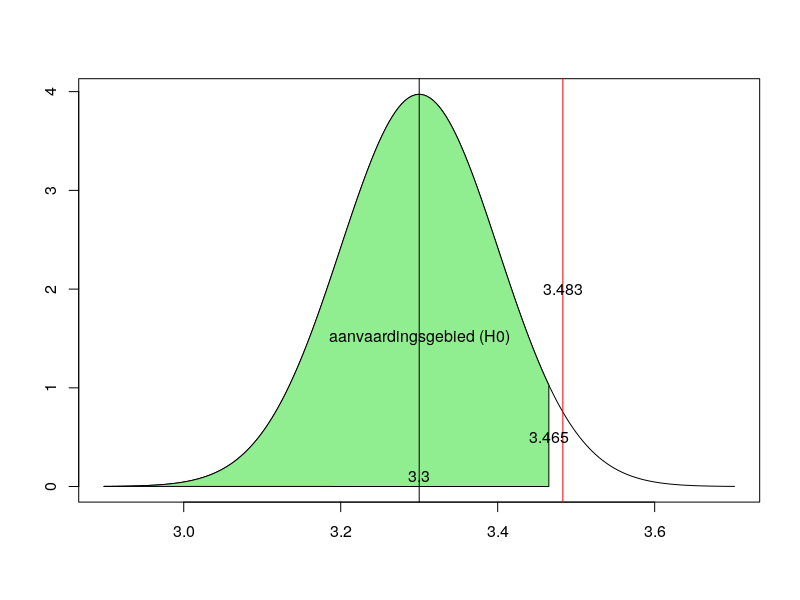
\includegraphics[width=\textwidth]{z-toets-reddingen}
  \caption{R Plot for the case study of Example~\ref{ex:hypothesis-test-daily-rescues}}
\end{figure}

\section{Examples}
\label{sec:testing-procedures-examples}

\begin{example}
  For a random sample consisting of 50 observations we have that:
  \begin{itemize}
    \item $\overline{x} = 25$
    \item $s = \sqrt{55} = 7,41$
  \end{itemize}
  
  We want to find out if there is a reason to assume that the popolation mean $\mu$ is smaller than 27.
  
  \begin{enumerate}
    \item Formulate both hypotheses. 
    
    $H_{0} : \mu = 27$ and $H_{1}: \mu < 27$.
    
    \item Determine significance level $\alpha$ and sample size $n$.
    
    $\alpha = 0.05$ and $n=50$.
    
    \item Calculate the value of the test statistic.
    
    For this we select the sample mean $M$. According to the central limit theorem, we have that:
    
    \[ M \sim Nor(\mu = 27, \frac{\sigma}{\sqrt{n}}) \]
    
    The test statistic is:
    \[ Z = \frac{\overline{x} - \mu}{\frac{\sigma}{\sqrt{n}}} = \frac{25-27}{\sqrt\frac{55}{50}} \approx -1.91\]
    
    \item Calculate the critical value.
    
    We discover a critical value for the mean of \texttt{pnorm(-1.91)} or about $0.0281$. Given a significance level of 0.05, this indicates that we can reject $H_{0}$.
    
    \item Calculate and plot the critical region.
    
    \[ g = \mu - z \times \frac{\sigma}{\sqrt{n}} \]
    
    and therefore:
    
    \[ g = 27 - 1.645 \times \sqrt{\frac{55}{50}} \]
    \[ g =  25.27470944 \]
    
    We discover that $\overline{x} < g$, and therefore we can make the same conclusion, to reject $H_{0}$.
    
  \end{enumerate}
\end{example}

\begin{example}
  In a reseach about the amount of change in the pockets of our superheroes, researchers state that on average a superhero carries 25 euro of cash.
  They assume that the population variance $\sigma = 7$.
  For a random sample of size $n=64$, the average amount of money a superhero carries is $\overline{x} = 23$ euro. 
  For the significance level, $\alpha = 0,05$ is selected.
  
  \begin{enumerate}
    \item Formulate both hypotheses.
    
    $H_{0} : \mu = 25$ and $H_{1}: \mu \neq 25$.
    
    \item Determine significance level $\alpha$ and sample size $n$.
    
    $\alpha = 0.05$ and $n=64$.
    
    \item Calculate the critical values.
    
    \[ g_{1} = \mu - z \times \frac{\sigma}{\sqrt{n}} = 23.28 \]
    
    \[ g_{2} = \mu + z \times \frac{\sigma}{\sqrt{n}} = 26.72 \]
    
    \item Critical region.
    
    We discover that $\overline{x}$ is inside the critical region (because $\overline{x} = 23 < g_1 = 23.28$), so we can reject $H_{0}$.
    
  \end{enumerate}
\end{example}

\section{The \texorpdfstring{$t$}{t}-test}
\label{sec:t-test}

For the $Z$-test there are a few assumptions that we need to take into account:

\begin{itemize}
  \item The sample size needs to be sufficiently large ($n \ge 30$);
  \item The test statistic needs to have a normal distribution;
  \item The variance of the population, $\sigma$, is known.
\end{itemize}
 
Because of these, we can apply the central limit theorem.

Sometimes these assumptions will not hold and therefore we can \emph{not} use the $Z$-test! In this scenario we can use the Student's $t$-distribution. However, note that the $t$-test\index{$t$-test}\index{test!$t$-} assumes that the investigated variable has a normal distribution.

The Student's $t$-distribution is named after statisticus William Sealy Gosset\index{Gosset, William Sealy}. He was working in the Guiness brewery and applied statistical methods to guarantee the quality of the beer. His employer considered this to be a company secret and did not allow Gosset to publish using his own name. Therefore, he used the pseudonym Student\index{Student}.

For the $t$-test, the formula to calculate the critical value is adjusted to: 

\begin{equation}
  g = \mu \pm t \times \frac{s}{\sqrt{n}}
  \label{eq:critical-value-t-test}
\end{equation}

To determine the corresponding $t$-value, we need the number of degrees of freedom, $n-1$.
To estimate the standard deviation, we use the sample standard deviation, $s$.

\begin{example}
  \label{ex:t-test-daily-rescues}

  Suppose the researchers from Example~\ref{ex:hypothesis-test-daily-rescues} were unable to take a sufficiently large sample due to time constraints, and only made $n = 25$ observations, with the same sample mean of $\overline{x} = 3.483$. The standard deviation of this sample is $ s = 0.55 $.
  
  Given these circumstances, can we still conclude for a same significance level $\alpha = 0.05$ that on average, superhereos rescue \emph{more} than 3.3 people a day?
  
  \begin{enumerate}
    \item Formulate both hypotheses.
    
      $H_{0} : \mu = 3.3$ en $H_{1}: \mu > 3.3$.
    
    \item Determine significance level $\alpha$ and sample size $n$.
    
    $\alpha = 0.05$ en $n=25$.
    
    \item Calculate the critical value.
    
    \[ g_{2} = \mu + t \times \frac{s}{\sqrt{n}} \approx 3.3 + 1.711 \times \frac{0.55}{\sqrt{25}} \approx 3.488 \]
    
    In R, the value of $t$ is calculated using \texttt{qt(1-a, df = n - 1)} (with \texttt{a} the significance level and \texttt{df} the number of degrees of freedom.)
    
    \item Conclusion.
    
    We have that $\overline{x} = 3.483$ is smaller than the critical value, and therefore is inside the region of acceptance. Therefore we do \emph{not} reject $H_{0}$.
  \end{enumerate}

  In other words, although the results are similar in our sample, we can not make the same conclusion. Because our sample is too small, there is greater uncertainty as to whether the value of the sample mean is extreme enough to reject the null hypothesis.
  
  The code example below is the elaboration of Example~\ref{ex:t-test-daily-rescues} in R.
\end{example}

\lstinputlisting{data/t-test.R}

\begin{figure}
  \centering
  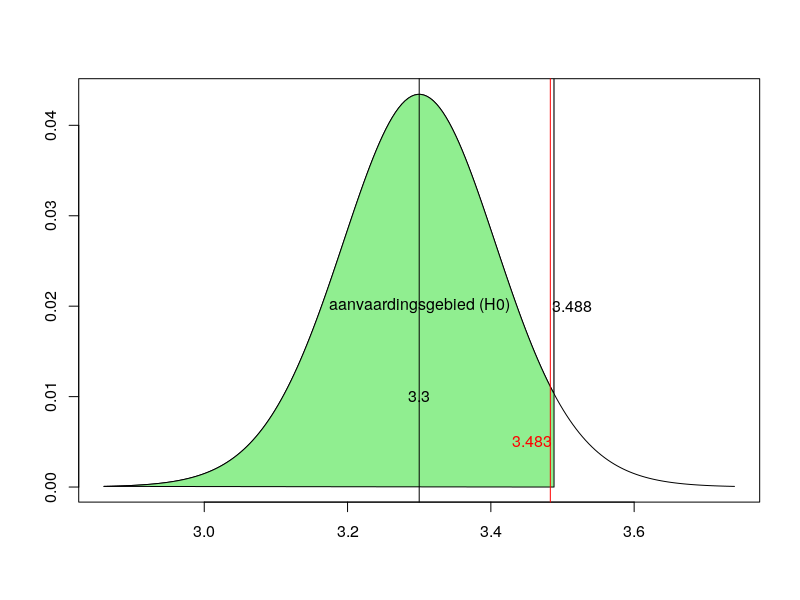
\includegraphics[width=\textwidth]{t-toets-reddingen}
  \caption{R Plot for the case study of Example~\ref{ex:t-test-daily-rescues}}
\end{figure}

\begin{example}
  An outbreak of a Salmonella-induced disease was attributed to vanilla ice cream from a particular factory~\autocite{Lindquist}.
  Scientists measured the level of Salmonella in 9 random samples.
  
  The levels (in MPN/g\footnote{Most Probable Number. See eg.~\url{http://www.microbiologie.info/mpn-methode.html} for more explanation about this method.}) are the following:
  
  \begin{center}
    \begin{tabular}{|l|l|l|l|l|}
      \hline
      0.593 & 0.142 & 0.329 & 0.691 & 0.231 \\ \hline
      0.793 & 0.519 & 0.392 & 0.418 &       \\ \hline
    \end{tabular}
  \end{center}

  Is there a reason to assume that the Salmonella level in the ice is significantly higher than 0.3 MPN/g? 
  We will use the R function \texttt{t.test} to answer this question.
  Read the help page of this function, to get an overview of all possible options.
  
  \begin{enumerate}
    \item Formulate both hypotheses.
    
    $H_0: \mu = 0.3, H_1: \mu > 0,3$
    
    \item Determine significance level $\alpha = 0.05$ and sample size $n = 9$. In R you need to use $1-\alpha = 0.95$.
    
    \item Calculate the probability value. This is a right-tailed test, which can be indicated in R using \texttt{alternative="greater"}. The selected confidence level is the default value of this function and therefore we don't need to add it explicitly.
    
\begin{lstlisting}
x <- c(0.593, 0.142, 0.329, 0.691, 0.231, 0.793, 0.519, 0.392, 0.418)
t.test(x, alternative = "greater", mu = 0.3)
\end{lstlisting}
    
    The result is:
    
\begin{verbatim}
One Sample t-test

data:  x
t = 2.2051, df = 8, p-value = 0.02927
alternative hypothesis: true mean is greater than 0.3
95 percent confidence interval:
0.3245133       Inf
sample estimates:
mean of x 
0.4564444 
\end{verbatim}
    \item Conclusion. The probability value $p = 0.029 < \alpha = 0.05$. Therefore we can reject the null hypothesis; in other words there is a strong indication that the average Salmonella level in the ice is greater than 0.3 MPN/g.
  \end{enumerate}
\textbf{Remark}: \texttt{``confidence interval: 0.3245133 Inf''} has no direct link with the region of acceptance or the critical region.
Is is also unrelated to the value $\mu_{0}=0.3$. 
It only indicates that because $\overline{x}=0.45644$,
we can say with 95\% confidence that the \textit{\'real\'} mean of the population ($\mu$) is between $0.3245133$ and $+\infty$.


See Section~\ref{ssec:confidence-interval-pop-mean-large-sample} (p.~\pageref{ssec:confidence-interval-pop-mean-large-sample}) and Section~\ref{ssec:confidence-interval-pop-mean-small-sample} (p.~\pageref{ssec:confidence-interval-pop-mean-small-sample}) for more information about confidence intervals.
\end{example}


\section{Errors in Hypothesis Tests}

In statistical hypothesis testing, errors can still occur. A type I error occurs when we reject a true null hypothesis $H_{0}$ (also known as a false positive). If we do not reject a false hypothesis $H_{0}$, we make a type II error (or false negative).

When performing a hypothesis test, the significance level $\alpha$ determines when exactly the null hypothesis can be rejected. Suppose we select a significance level of 5\%.
If the null hypothesis is true, the probability of taking a sample in the region of rejection is 5\%. 
In other words, the probability of rejecting a true null hypothesis is 5\%, or in general: the significance level of a test is equal to the probability of making a type I error.

Obviously, we want to minimize the risk of making a type I error.
Unfortunately, this is at the cost of a higher chance of making a type II error, denoted by $\beta$.
The relationship between $\alpha$ and $\beta$ is not trivial and out of scope for this course.

In many cases a type I error is worse than a type II error.
Think of a lawsuit where the null hypothesis states that the person is innocent.
If we test using a confidence level of 5\%, the probability of making a type I error is 5 out of 100.
In other words, there is a confidence of 95\% that the correct decision is made if $H_{0}$ is correct.
Because of this we try to avoid the conclusion that $H_{0}$ is accepted, 
but rather that the sample contains insufficient evidence to reject $H_{0}$ for a given significance level.

\begin{table}
  \centering
  \begin{tabular}{@{}l|cc@{}}
    \toprule
    & \multicolumn{2}{c}{\textbf{Reality}} \\
    \textbf{Decision}             & \textbf{$H_{0}$ True} & \textbf{$H_{1}$ True}     \\
    \midrule
    \textbf{$H_{0}$ not rejected} & Correct                       & Type II error (false negative) \\
    \textbf{$H_{0}$ rejected}     & Type I error (false positive) & Correct            \\
    \bottomrule
  \end{tabular}
  \caption{Conclusions and consequences when thesting a hypothesis; error types.}
  \label{tab:hypfouten}
\end{table}

\section{Exercises}
\label{sec:testing-procedures-exercises}

Source files for these exercises can be found in the Github repo, folder \texttt{exercises/datasets/}.



\begin{exercise}
  \label{ex:binding-recommendation}
  
  It is being said that introducing a ``binding recommendation on continuation of studies'' (refusing enrollment in the next academic year if a student did not complete a certain level of credits) has a positive effect on the study efficiency and success rate. Before the introduction of binding recommendations, the number of completed credits per student per year was 44 with a standard deviation of 6.2. After the introduction, a sample of 72 random students has an average number of completed credits of 46.2.
  
  \begin{enumerate}
    \item Test whether there is evidence that the introduction of binding recommendations has improved the success rate among students. Calculate the critical value for a significance level of $\alpha = 2.5\%$.
    \item Do the same by calculating the $p$-value.
    \item Explain what $\alpha = 2.5 \%$ means.
  \end{enumerate}
\end{exercise}

\begin{exercise}
  \label{ex:price-difference-cars}
  
  One of the motives for choosing a car dealership is the resale value of the previous car, or more specifically the price a dealer wants to pay for the old car when the customer buys a new one. The importer of Ford wants that all dealers implement the same price policy. The importer is of the opinion that the average price difference between the closest Ford dealer and the dealer where the old car was purchased should be at most \euro{300}. It is assumed that, if the difference is larger, potential customers will be more inclined to stay with their previous dealer.
  
  In a random sample, the following price differences are recorded:
  
  \begin{center}
    \begin{tabular}{|l|l|l|l|l|l|l|}
      \hline
      400 & 350 & 400 & 500 & 300 & 350 & 200 \\ \hline
      500 & 200 & 250 & 250 & 500 & 350 & 100 \\ \hline
    \end{tabular}
  \end{center}

  Test whether there is reason to assume that the average price difference in reality is significantly greater than \euro{300}, using a significance level of 5\%.
  
\end{exercise}

\begin{exercise}
  \label{ex:z-test-rlanders}
  Import the dataset \texttt{rlanders-generated.csv}~\footnote{This dataset was generated using \url{https://rlanders.net/dataset-generator/}} in R.
  
  The variable \emph{Money} represents a gross annual salary ($\times 100\$$). We assume this variable has a mean of $\mu = 490$ with standard deviation $\sigma = 98$. If we calculate the sample mean over the total dataset (do it yourself!), it seems to support our assumptions. But what if we looked at men and women separately (variable \emph{Gender})?
  
  Use an appropriate statistical test to verify the statements below, usinge a significance level of $\alpha = 5\%$.
  For each statement, calculate the critical value(s) and the p-value.
  
  \begin{enumerate}
    \item The average gross annual salary of men seems \emph{higher} than the average. Is it also significantly higher?
    \item The average gross annual salary of women seems \emph{lower}. Is it significantly lower?
    \item Calculate the region of acceptance for the average gross annual salary for the sample (men and women combined). In this case we want to verify if the sample mean is significantly different from the expected value, but it can be lower or higher.
  \end{enumerate}
  
\end{exercise}

\subsection{Solutions to selected exercises}
\label{sec:testing-procedures-solutions}

\paragraph{Exercise~\ref{ex:critical-value-left-tail}:}

\begin{equation}
g = \mu - z \times \frac{\sigma}{\sqrt{n}}
\label{eq:kritiekeRechtseWaarde2}
\end{equation}

because

\[ P(M < g) = P\left(Z < \frac{g - \mu}{\frac{\sigma}{\sqrt{n}}}\right) = 0,05 \]

Thanks the symmetry rule, we know that:
\[ P\left(Z > - \left( \frac{g - \mu}{\frac{\sigma}{\sqrt{n}}} \right) \right) = 0,05 \]

The corresponding z-value is 1.645, and therefore:
\[ z = \frac{-g + \mu}{\frac{\sigma}{\sqrt{n}}} \]
\[ \Leftrightarrow -g = \frac{\sigma}{\sqrt{n}} z - \mu \]
\[ \Leftrightarrow g = -\frac{\sigma}{\sqrt{n}} z + \mu \]

\paragraph{Exercise~\ref{ex:binding-recommendation}}

\begin{enumerate}
  \item $g \approx 45.4 < \overline{x} = 46.2$.
  
  $\overline{x}$ is inside the critical region, so we can reject the null hypothesis. Therefore, we can assume that binding recommendation on continuation of studies does increase the success rate.
  
  \item $P(M > 46.2) \approx 0.0013 < \alpha = 0.025$. The probability value is smaller than the significance level, so we can reject the null hypothesis.
  
  \item  $\alpha$ is the probability of rejecting a true null hypothesis $H_{0}$. In other words, there is a 2.5\% chance that you wrongly conclude that the success rate has increased.
\end{enumerate}

\paragraph{Exercise~\ref{ex:price-difference-cars}}

In this context ($n = 14 < 30$) the $z$-test cannot be used. Instead, we use Student's $t$-test.

\begin{itemize}
  \item $\overline{x} \approx 332.143$
  \item $s \approx 123.424$
  \item $g \approx 358.42$. The sample mean is outside of the critical region, so we cannot reject $H_0$.
  \item $p \approx 0.1738$. $p \nless \alpha$, so we cannot reject $H_0$.
\end{itemize}

Based on this sample there is no reason to assume that the average price difference on the residual value of old cars is significantly greater than the amount recommended by the importer.

\paragraph{Exercise~\ref{ex:z-test-rlanders}}

The mean of the whole sample is $\overline{x} \approx 501.156$

\begin{enumerate}
  \item Only men (right-tailed $Z$-test):
    \begin{itemize}
      \item $\overline{x}_m \approx 507.535$
      \item $g_m \approx 511.456$
      \item $p_m \approx 0.1396$
      \item We \textit{cannot} reject the null hypothesis. The average gross annual salary of men is the sample is not significantly higher than the average.
    \end{itemize}
  \item Only women (left-tailed $Z$-test):
    \begin{itemize}
      \item $\overline{x}_f \approx 472.058$
      \item $g_f \approx 477.646$
      \item $p_f \approx 0.0199$
      \item We \text{can} reject the null hypothesis. The average gross annual salary of women in the sample is significantly lower than the average.
    \end{itemize}
  \item The region of acceptance corresponds to the interval [487.852; 512.148].
\end{enumerate}
